\subsection{Database}

As the database of the server is quite complex, we have divided the drawings, so
that we have one drawing per module.

\subsubsection{Core}

The core database-architecture used for storing the rules is described in
figure \ref{fig:server_database_core}. 

\begin{figure}[h]
        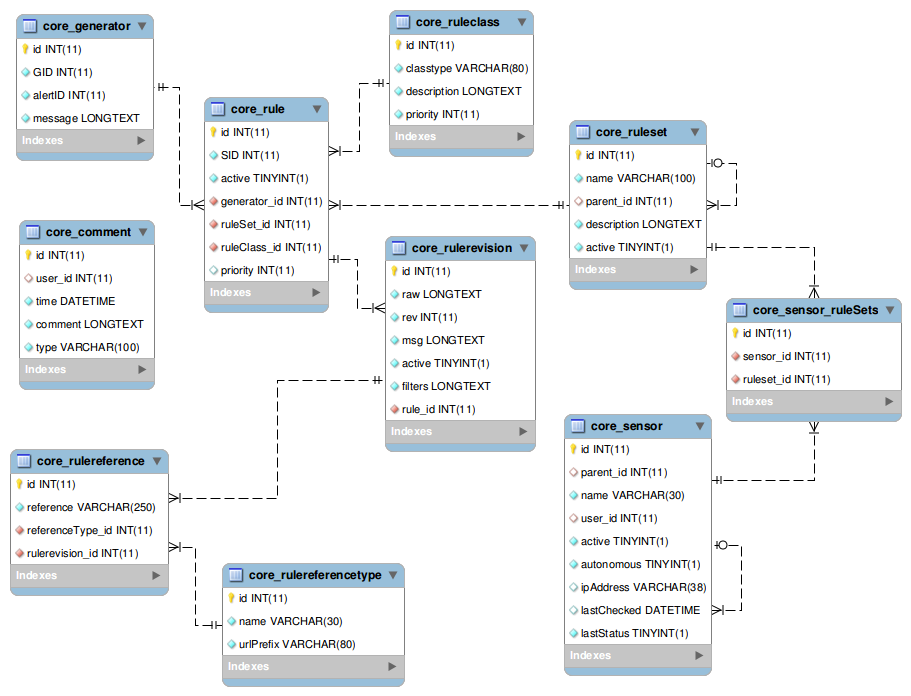
\includegraphics[width=127mm]{./img/Server-DB-Core.png}
        \caption{Core server-database}
        \label{fig:server_database_core}
\end{figure}

The most central part of our system is the representation of a Rule. A single
Rule might have several Revisions, as we might want to keep some history when
they get updated. Each Revision have its own set of References attached.

A single Rule also have a lot of other properties which it might share with
other Rules. A Generator, a Classification and a Ruleset are examples of such.

Finally, the Rules are assigned to a Sensor by attaching Rulesets to the
Sensor.

\subsubsection{Tuning}

In addition to storing the raw rules, we would like to be able to store
tuning parameters on the rules. As sensors might have different
tuning parameters, we cannot attach the tuning directly to the rules. Separate
tables (as described in figure \ref{fig:server_database_tuning}) is thus needed
to model the tuning parameters.

\begin{figure}[h]
        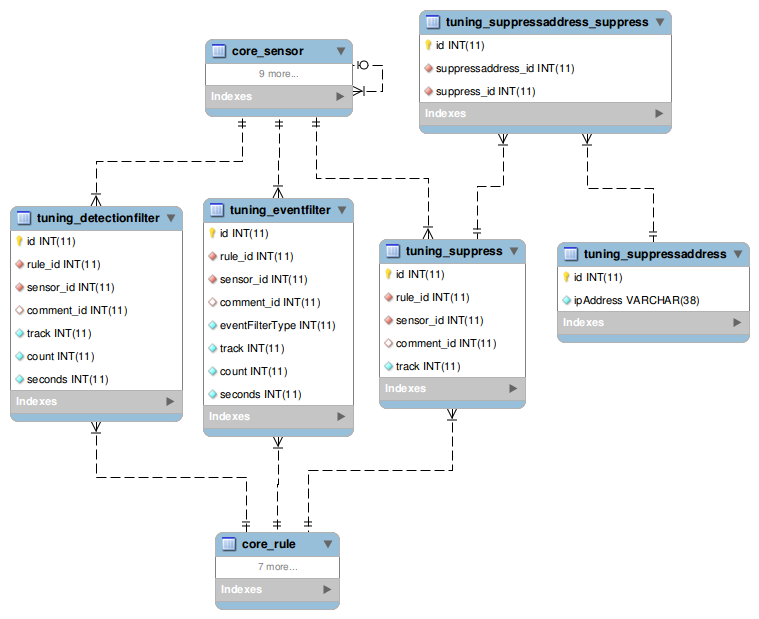
\includegraphics[width=127mm]{./img/Server-DB-Tuning.png}
        \caption{Tuning server-database}
        \label{fig:server_database_tuning}
\end{figure}

Both types of filters, and the suppressions are connected to a Rule and a
Sensor. This way, we let the user spesify filters for the individual sensors.
If a sensor does not have a filter applied, but any parent sensor of that sensor
has one, the closest parent's filter will be applied.

\subsubsection{Update}

When rules are inserted to the database, we would like to have some traceability
to be able to determine where and when a rule has entered our system. To be
able to do this, we have the update object (figure
\ref{fig:server_database_update}).

\begin{figure}[h]
        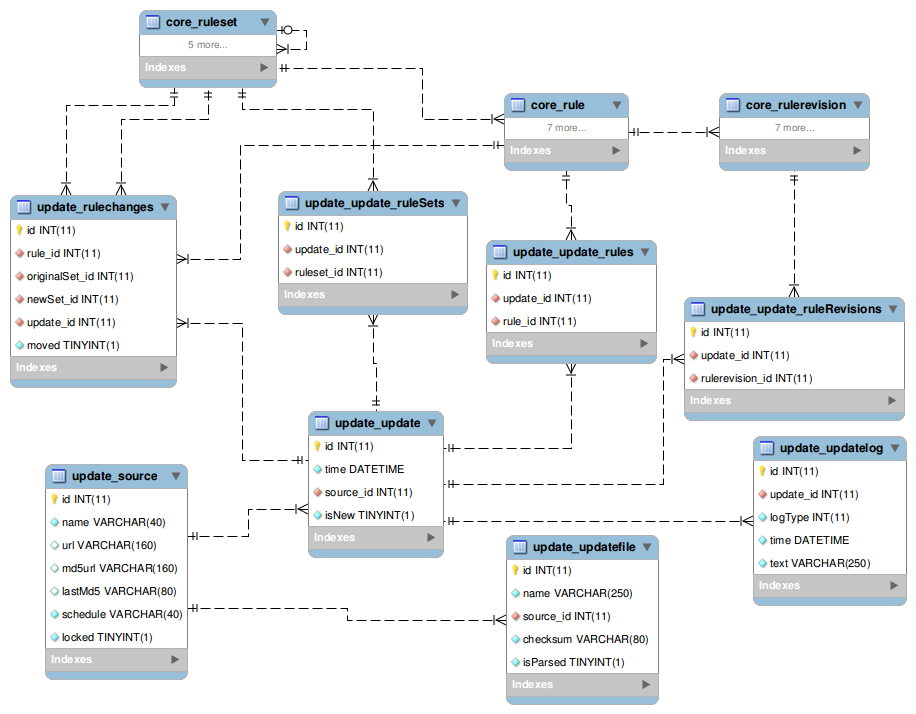
\includegraphics[width=127mm]{./img/Server-DB-Update.png}
        \caption{Update server-database}
        \label{fig:server_database_update}
\end{figure}

The structure of update lets us store the update sources,
and add an update object for each update ran from a given source. These update
objects can in turn have relations to rules, rulesets and rulerevisions, so
that we can track changes for each update.